\chapter{Storage in lakes and reservoirs} \label{chap:resStor}
\renewcommand{\tabdir}{chapters/part_processes/reservoirStorage/tab}
\renewcommand{\figdir}{chapters/part_processes/reservoirStorage/fig}

\section{Introduction} \label{sec:resStor_intro}

This chapter desribes approaches to the simulation of water storage in reservoirs. In a wider sense, the term \emph{reservoir} includes natural lakes and the various types of operated reservoirs.

%%%%%%%%%%%%%%%%%%%%%%%%%%%%%%%%%%%%%%%%%%%%%%%%%%%%%%%%%%%%%%%%%%%%%%%%%%%%%%%%
%%%%%%%%%%%%%%%%%%%%%%%%%%%%%%%%%%%%%%%%%%%%%%%%%%%%%%%%%%%%%%%%%%%%%%%%%%%%%%%%
%%%%%%%%%%%%%%%%%%%%%%%%%%%%%%%%%%%%%%%%%%%%%%%%%%%%%%%%%%%%%%%%%%%%%%%%%%%%%%%%

\section{Storage in uncontrolled lakes} \label{sec:resStor_lake}

%%%%%%%%%%%%%%%%%%%%%%%%%%%%%%%%%%%%%%%%%%%%%%%%%%%%%%%%%%%%%%%%%%%%%%%%%%%%%%%%

\subsection{Processes and equations} \label{sec:resStor_lake_processes}

The fundamental principle for the simulation of lake storage is expressed by the mass balance equation (\eqnref{eqn:resStor_lake_massBalancePure}).

\begin{equation} \label{eqn:resStor_lake_massBalancePure}
  \frac{dv}{dt} = q_{in} + p - q_{out} - e
\end{equation}

\begin{tabular}{lll}
  $v$ & Storage volume & L$^3$ \\
  $q_{in}$ & Inflow rate & L$^3$/T \\
  $q_{out}$ & Outflow rate & L$^3$/T \\
  $p$ & Precipitation flux & L$^3$/T \\
  $e$ & Evaporation flux & L$^3$/T \\
\end{tabular}

\medskip
For a natural lake with a single outflow, the outflow rate is related to the lake's water level $h$ through a rating curve $Q_{out}(h)$ (\figref{fig:resStor_lake_massBalance}). Furthermore, the water level $h$ is related to the storage volume $v$ by the storage curve $H(v)$. The latter represents the lake's bathymetry, \ie{} the topography of the bottom. Sometimes, the rating curve and the storage curve may be represented by analytical functions, typically using power equations or polynomials, respectively. In practice, however, lookup tables generally allow for greater flexibility as compared to analytical expressions.

\begin{figure}
  \centering
  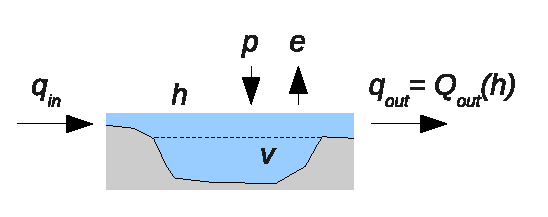
\includegraphics[width=0.7\columnwidth]{\figdir/balance.eps}
  \caption[Side view of a lake with uncontrolled outflow through an outlet channel.]{Side view of a lake with uncontrolled outflow through an outlet channel. Symbols as in \eqnref{eqn:resStor_lake_massBalancePure}. \label{fig:resStor_lake_massBalance}}
\end{figure}

The rates of precipitation and evaporation fluxes are obtained by multiplying the corresponding rates (dimension L/T) with an appropriate value of the lake's surface area (\eqnref{eqn:resStor_lake_fluxP} \& \ref{eqn:resStor_lake_fluxE}).

\begin{align}
p= & P \cdot a_{max}  \label{eqn:resStor_lake_fluxP} \\
e= & E \cdot A(H(v))  \label{eqn:resStor_lake_fluxE}
\end{align}

\begin{tabular}{lp{0.5\columnwidth}l}
  $P$ & Intensity of precipitation & L/T \\
  $E$ & Rate of evaporation & L/T \\
  $a_{max}$ & Maximum extent of the lake's surface area & L$^2$ \\
  $A(h)$ & Surface area as a function of water level $h$ & L$^2$ \\
\end{tabular}

\medskip
The reasons for using different values of the surface area in the calculation of precipitation and evaporation fluxes are as follows:
\begin{itemize}
  \item If a constant surface area would be used in \eqnref{eqn:resStor_lake_fluxE}, this would no longer be a continuous function. As long as the there was some water in the lake, the evaporation flux would be $>0$. But as soon as the last amount of liquid water has vanished, the flux becomes zero. Such a discontinuity is problematic when solving the differential equation \eqnref{eqn:resStor_lake_massBalancePure}. The choice of a \emph{continuous} function $A(h)$ resolves this problem, as it makes the evaporation flux $E$ decrease gradually, as the storage volume approaches zero.
  \item In reality, the lake's surface area being exposed to precipitation is variable too, as expressed by $A(h)$. However, in hydrological catchment models, the area of \emph{land surfaces} is typically constant. Therefore, to avoid mass balance errors, the lake's surface area is taken as constant too. The maximum extent of the lake $a_{max}$ is a natural choice. Effectively, rain falling on possibly dry parts of the bottom still contributes to the lake's storage volume.
\end{itemize}

Using the rating curve $Q_{out}(h)$ and the storage curve $H(v)$ as well as the definitions from \eqnref{eqn:resStor_lake_fluxP} and \ref{eqn:resStor_lake_fluxE}, the mass balance (\eqnref{eqn:resStor_lake_massBalancePure}) can be rewritten as \eqnref{eqn:resStor_lake_massBalanceExt}.

\begin{equation} \label{eqn:resStor_lake_massBalanceExt}
  \frac{dv}{dt} = q_{in} + P \cdot a_{max} - Q_{out}(H(v)) - E \cdot A(H(v))
\end{equation}

%%%%%%%%%%%%%%%%%%%%%%%%%%%%%%%%%%%%%%%%%%%%%%%%%%%%%%%%%%%%%%%%%%%%%%%%%%%%%%%%

\subsection{Mathematical solution} \label{sec:resStor_lake_solution}

\subsubsection*{Strategy}
The two functions $Q_{out}(H(v))$ and $A(H(v))$ at the right hand side of \eqnref{eqn:resStor_lake_massBalanceExt} may be arbitrarily complicated. Moreover, the functions are typically available as lookup tables rather than analytical expressions. Therefore, \eqnref{eqn:resStor_lake_massBalanceExt} has to be solved numerically. To obtain accurate and stable (\ie{} positive) solutions, an ODE solver with automatic time-step adjustment must be used.

\subsubsection*{Inflow rates}
The currently used implementation allows for a linear variation of the inflow rate within a discrete modeling time step of length $\Delta t$. As input, the time-step averaged inflow rate $\overline{q_{in}}$ and the instantaneous rate at the end of the time step $q_{in}(t_0 + \Delta t)$ are used. The missing rate at the begin of the time step $q_{in}(t_0)$ is estimated as described in \secref{sec:chanFlow_singleRes_solution} (page~\pageref{sec:chanFlow_singleRes_solution}).

\subsubsection*{Outflow rates}
The numerical solution of \eqnref{eqn:resStor_lake_massBalanceExt} yields the storage volume at the end of a modeling time step and the corresponding outflow rate $q_{out}(t_0 + \Delta t)$ is obtained from the combined rating curve and storage curve $Q_{out}(H(v))$.

An accurate time-step averaged outflow rate $\overline{q_{out}}$ is calculated from a discrete version of the mass balance equation (\eqnref{eqn:resStor_lake_outflowAvg}).

\begin{equation} \label{eqn:resStor_lake_outflowAvg}
  \overline{q_{out}}= \frac{v(t_0) - v(t_0 + \Delta t)}{\Delta t} + \overline{q_{in}} + \frac{vp}{\Delta t} - \frac{ve}{\Delta t}
\end{equation}

Here, $vp$ and $ve$ represent the total volumes of precipitation input and evaporation losses within a single time step, respectively. Both $vp$ and $ve$ are treated as state variables which are initialized to zero at the beginning of a time step ($t_0$). This approach allows for the computation of a proper mass balance even if the rates of precipitation or evaporation are variable over $\Delta t$. Currently, this is only the case for evaporation, since the flux is dependend on the storage (see \eqnref{eqn:resStor_lake_fluxE}).

%%%%%%%%%%%%%%%%%%%%%%%%%%%%%%%%%%%%%%%%%%%%%%%%%%%%%%%%%%%%%%%%%%%%%%%%%%%%%%%%

\subsection{Implementation} \label{sec:resStor_lake_implementation}

\tabref{tab:resStor_lake_implementation} relates the identifier names used in the model implementation (names of state variables, parameters, inputs, and outputs) to the symbols used in the process equations (\secref{sec:resStor_lake_processes}). Note that this table does not list external input variables used in the calculation of the rate of evaporation (symbol $E$ in \eqnref{eqn:resStor_lake_fluxE}). Modeling concepts for evaporation can be found in \chapref{chap:evap}.

\begin{table*}
\caption{Symbols used in the process equations (\secref{sec:resStor_lake_processes}) and corresponding identifiers. \label{tab:resStor_lake_implementation}}
\begin{tabular}{|p{0.2\textwidth}p{0.13\textwidth}p{0.07\textwidth}p{0.42\textwidth}|}  \hline
\rowcolor[gray]{0.9}
Symbol & Identifier & Units & Details \\ \hline
\multicolumn{4}{|c|}{\textit{State variables}} \\
$v$ & \verb!v! & \cbm{} & Storage volume \\
$vp$ & \verb!vp! & \cbm{} & Total volume of precipitation in a single time step \\
$ve$ & \verb!ve! & \cbm{} & Total evaporated volume in a single time step \\ \hline
\multicolumn{4}{|c|}{\textit{Simulated inputs}} \\
$\overline{q_{in}}$ & \verb!qi_avg! & \cbm{}/s & Inflow rate (time-step average) \\
$q_{in}(t_0 + \Delta t)$ & \verb!qi_end! & \cbm{}/s & Inflow rate (value at end of time-step) \\  \hline
\multicolumn{4}{|c|}{\textit{Scalar parameters (object-specific)}} \\
$a_{max}$ & \verb!area_max! & \sqm{} & Maximum surface area \\  \hline
\multicolumn{4}{|c|}{\textit{Parameter functions (object-specific)}} \\
$H(v)$ & \verb!v2h! & m & Storage curve (tabulated function) \\
$A(h)$ & \verb!h2a! & \sqm{} & Area curve to compute evaporation loss (tabulated function) \\
$Q_{out}(h)$ & \verb!h2q! & \sqm{} & Rating curve at lake outlet (tabulated function) \\  \hline
\multicolumn{4}{|c|}{\textit{Outputs}} \\
$\overline{q_{out}}$ & \verb!qx_avg! & \cbm{}/s & Outflow rate (time-step average) \\
$q_{out}(t_0 + \Delta t)$ & \verb!qx_end! & \cbm{}/s & Outflow rate (value at end of time-step) \\
$h$ & \verb!h! & m & Water level \\ \hline
\end{tabular}
\end{table*}


%%%%%%%%%%%%%%%%%%%%%%%%%%%%%%%%%%%%%%%%%%%%%%%%%%%%%%%%%%%%%%%%%%%%%%%%%%%%%%%%

\section{Notes on input data} \label{sec:resStor_inputs}

In real-world model applications, the required functions $H(v)$, $Q_{out}(h)$, and $A(h)$ are often not known but have to be estimated. Some recommendations are given in the sub-sections below.

\subsection{Storage curve}
Sometimes, information on the lake's bathymetry are available from topographic maps as lines of equal depth. Via the steps of digitizing and vector-to-raster conversion, a digital elevation model (DEM) of the lake's bottom can be obtained using GIS. Alternatively, the DEM can be obtained by interpolation of punctual measurements. The inverse of the storage curve $H(v)$ can be calculated using \eqnref{eqn:resStor_storageCurveFromDEM}.

\begin{equation}
V(h)= (\Delta x)^2 \cdot \sum_{i=1}^{nx} \sum_{k=1}^{ny} max(0, h - z(i,k)) \label{eqn:resStor_storageCurveFromDEM}
\end{equation}

\begin{tabular}{lp{0.6\columnwidth}l}
  $V(h)$ & Storage volume corresponding to water level $h$ & L$^3$ \\
  $(\Delta x)^2$ & Area of a single raster cell & L$^2$ \\
  $nx, ny$ & Number of cells in x- and y-direction (grid dimensions) & -- \\
  $z(i,k)$ & Elevation of the bottom at cell with indices $i$ and $k$ & L \\
\end{tabular}

\medskip
The evaluation of \eqnref{eqn:resStor_storageCurveFromDEM} for discrete values of $h$ yields a lookup table for $V(h)$. The desired function $H(v)$ is then obtained by inverting $V(h)$. Usually, it makes sense to apply some kind of interpolation in order to tabulate $H(v)$ for a reasonable set of arguments $v$.

For operational model applications, it is important that the table $H(v)$ covers the highest thinkable values of the storage volume $v$. Otherwise, the model might stop just in the moment where it is needed the most. The choice of a lower limit for $v$ is site-specific. Given that the outflow of the lake never runs dry, it is sufficient if the smallest tabulated value of $H(v)$ corresponds to the lowest point of the channel at the lake's outlet (dashed horizontal line in \figref{fig:resStor_lake_massBalance}). However, if the water level can fall below this level due to high evaporation (causing the outflow rate to be exactly zero), the table $H(v)$ must also cover those states.

\subsection{Surface area curve}
The function $A(h)$ can be obtained from a DEM as well using \eqnref{eqn:resStor_areaCurveFromDEM}. By convention, the logical expression $(h > z(i,k))$ equals 1 if true and it is 0 otherwise.

\begin{equation}
A(h)= (\Delta x)^2 \cdot \sum_{i=1}^{nx} \sum_{k=1}^{ny} (h > z(i,k)) \label{eqn:resStor_areaCurveFromDEM}
\end{equation}

It is sufficient if $A(h)$ is tabulated for the range of $h$ values which are expected to appear during simulation (including extremes). For lakes which can fall dry, it is important that $A(h)$ is continuous, \ie{} the value should \emph{gradually} approach zero for values of $h$ which correspond to minimal storage volumes. In other words, the lake's bottom must not be perfectly flat.

\subsection{Rating curve (uncontrolled lakes)}

For natural lakes, the rating curve $Q_{out}(h)$ can be estimated from the characteristics of the outlet channel using Mannings's equation (see \eqnref{eqn:chanFlow_singleRes_manning} at page~\pageref{eqn:chanFlow_singleRes_manning}). The required information include the cross-section's geometry, the slope of the bottom, and the roughness (Manning's $n$).

For the special case of a channel whose width $W$ is much greater than the flow depth $h_{fl}$, the hydraulic radius is approximatekly equal to $h_{fl}$. Then, Mannings's equation simplifies to \eqnref{eqn:resStor_manningWideChannel}.

\begin{equation} \label{eqn:resStor_manningWideChannel}
  q(h_{fl})= \frac{1}{n} \cdot \sqrt{S_f} \cdot h_{fl}^{5/3} \cdot W
\end{equation}
\medskip
\begin{tabular}{lll}
  $q$ & Flow rate & \cbm/s \\
  $S_f$ & Slope of the energy grade line & -- \\
  $h_{fl}$ & Flow depth (x-section average) &  m \\
  $W$ & Channel width & m \\
  $n$ & Manning's $n$ (parameter) & Non-physical \\
\end{tabular}
